
    \documentclass[tikz,convert={outfile=\jobname.png}]{standalone}
    \usetikzlibrary{mindmap,trees,backgrounds}
    \usepackage{fontspec}
    \defaultfontfeatures{Ligatures=TeX,Scale=3}
    \setmainfont{M+ 1mn}
    
    
    \definecolor{brightube}{RGB}{209.1, 158.1, 232.05}
    \definecolor{cobalt}{RGB}{0.0, 71.4, 170.85000000000002}
    \definecolor{deeppink}{RGB}{255.0, 20.400000000000002, 147.89999999999998}
    \definecolor{saffron}{RGB}{244.79999999999998, 196.35, 48.45}
    \definecolor{tealblue}{RGB}{53.55, 117.30000000000001, 135.15}
    \definecolor{tigerseye}{RGB}{224.4, 140.25, 61.199999999999996}
    \definecolor{yellow-green}{RGB}{153.0, 204.0, 51.0}
    \definecolor{white}{RGB}{255.0, 255.0, 255.0}
    \definecolor{dimgray}{RGB}{104.55, 104.55, 104.55}
    
    \begin{document}
    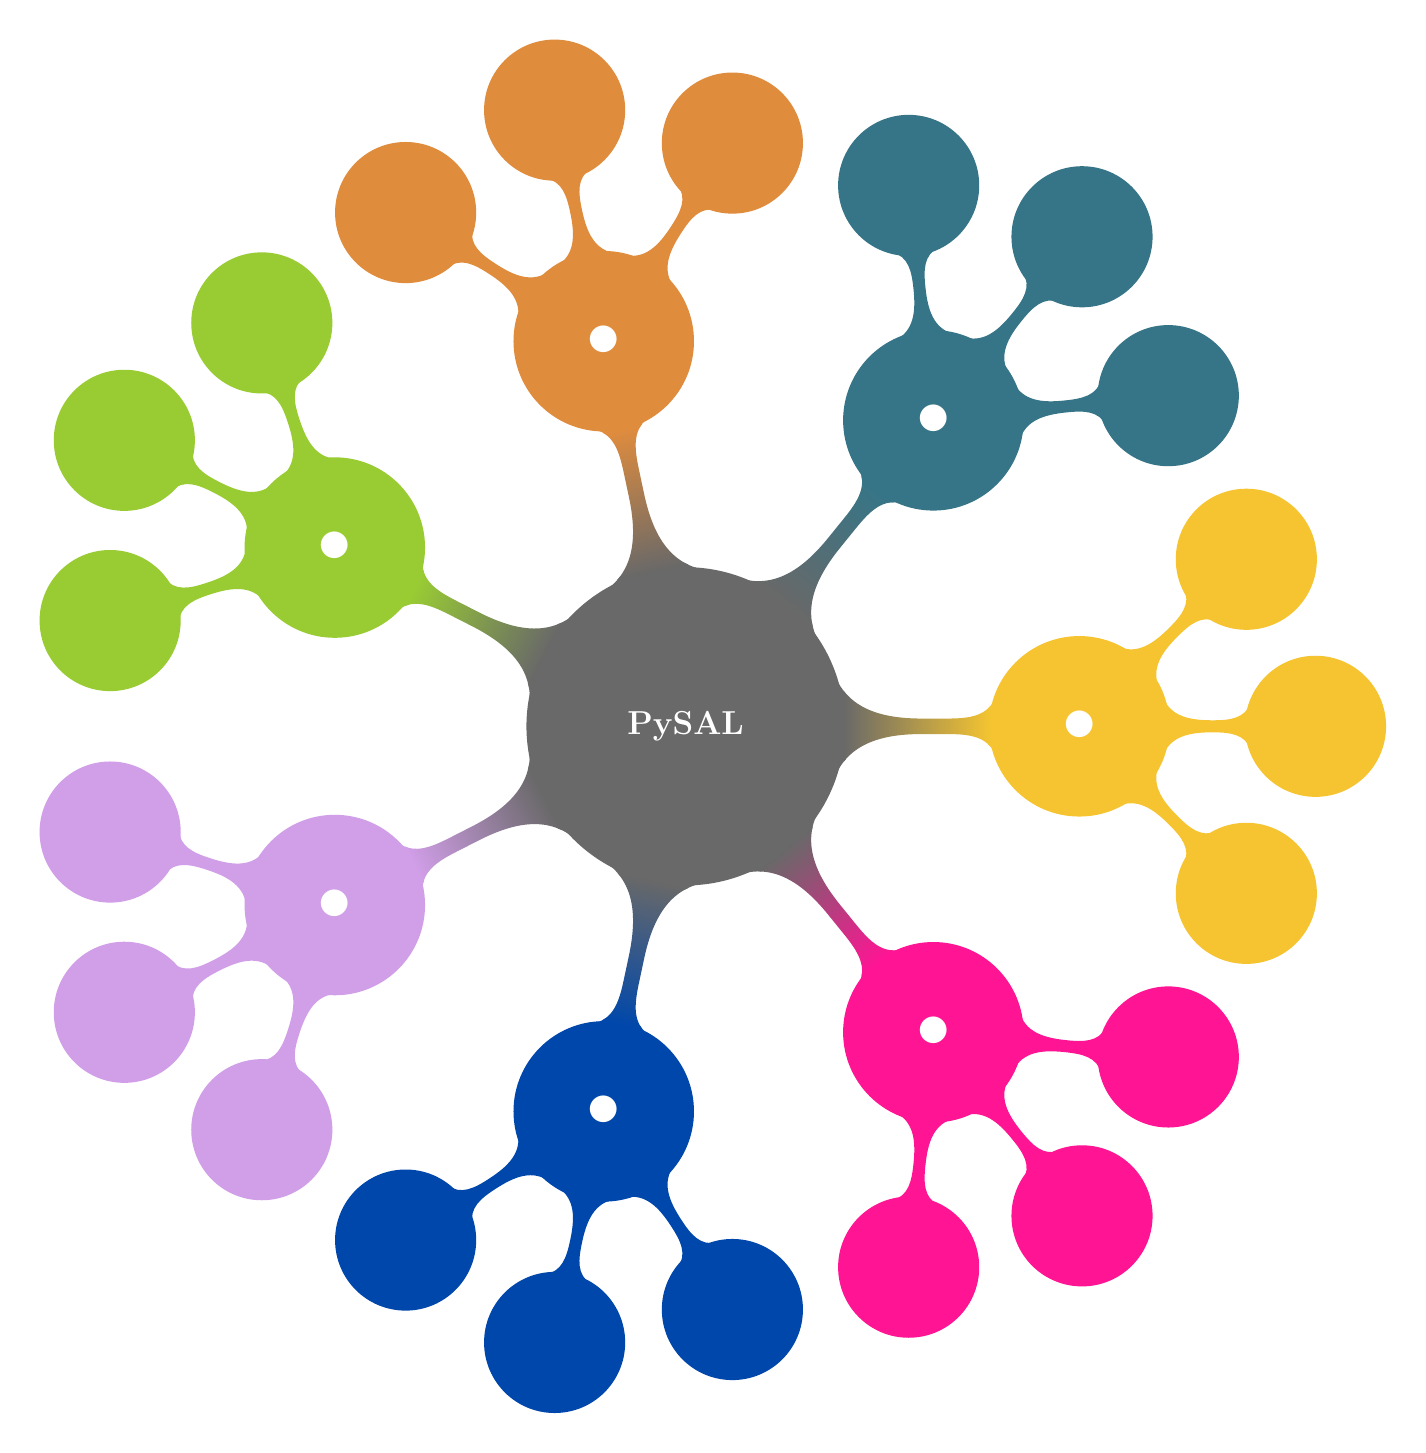
\begin{tikzpicture}[
        background rectangle/.style={fill=white},
        show background rectangle,
        mindmap,
        grow cyclic,
        every node/.style=concept,
        concept color=dimgray,
        text=white,
        level 1/.append style={
            level distance=5cm,
            sibling angle=51,
            font=\Huge
        },
        level 2/.append style={
            level distance=3cm,
            sibling angle=45
        }
    ]
    
        \node[concept color=dimgray]{\large\bfseries{PySAL}}
        child [concept color=brightube]{ node {$\bullet$}
            child { node { }}
            child { node { }}
            child { node { }}
         }
        child [concept color=cobalt]{ node {$\bullet$}
            child { node { }}
            child { node { }}
            child { node { }}
         }
        child [concept color=deeppink]{ node {$\bullet$}
            child { node { }}
            child { node { }}
            child { node { }}
         }
        child [concept color=saffron]{ node {$\bullet$}
            child { node { }}
            child { node { }}
            child { node { }}
         }
        child [concept color=tealblue]{ node {$\bullet$}
            child { node { }}
            child { node { }}
            child { node { }}
         }
        child [concept color=tigerseye]{ node {$\bullet$}
            child { node { }}
            child { node { }}
            child { node { }}
         }
        child [concept color=yellow-green]{ node {$\bullet$}
            child { node { }}
            child { node { }}
            child { node { }}
         }
                ;
    \end{tikzpicture}
    \end{document}